\begin{figure*}
  \begin{center}

    \hspace*{-4em}
    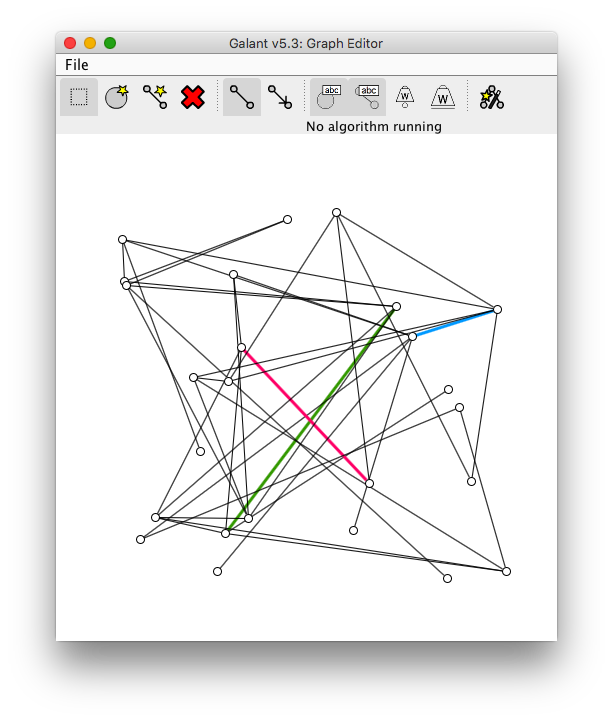
\includegraphics[width=0.375\textwidth]{X-r_25_40_1}
    \hspace{-2em}
    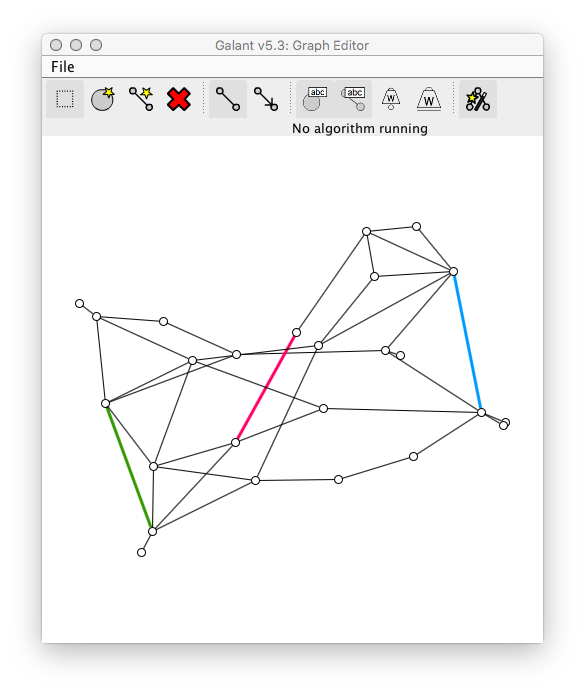
\includegraphics[width=0.375\textwidth]{X-r_25_40_1-fd}
    \hspace{-2em}
    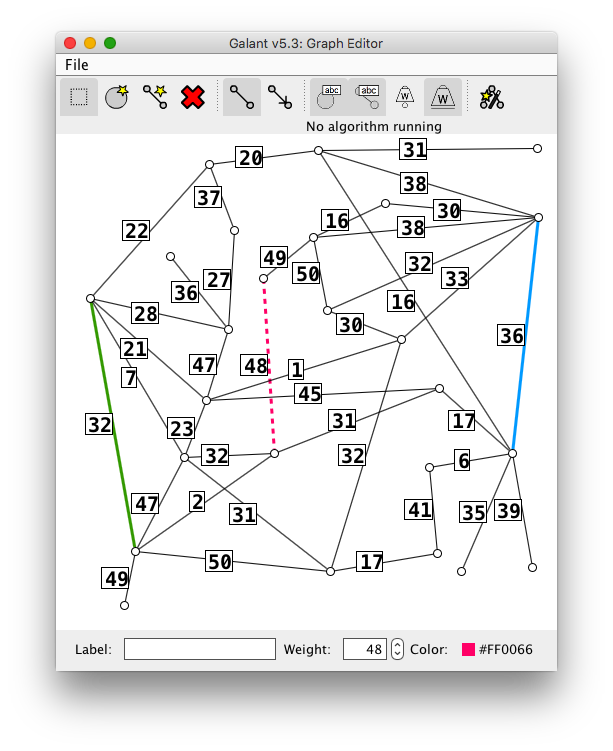
\includegraphics[width=0.375\textwidth]{X-r_25_40_1-edited}

    \hspace*{-4em}
    \parbox[c][3ex][c]{0.35\textwidth}{
      (a) A graph from an external random generator.
    }
%    \hspace{-2em}
    \parbox[c][3ex][c]{0.35\textwidth}{
    (b) Force directed layout applied.
    }
%    \hspace{-2em}
    \parbox[c][3ex][c]{0.35\textwidth}{
    (c) User moved nodes for an even better layout.
    }

  \end{center}

  \bigskip
  \caption{Using force directed drawing to lay out graphs for more convenient
    editing and more compelling animations. Node ids do not appear because
    a node radius of~3 was specified using the
    \Code{Preferences$\rightarrow$Graph~Display} panel.}

  \label{fig:force_directed}
\end{figure*}

% [Last modified: 2017 01 06 at 01:42:15 GMT]
